% !Mode:: "TeX:UTF-8"
\title{实验四 HDFS的Java API操作 实验报告}
\author{江昱峰 21009200038} 
\documentclass {article}
\usepackage[UTF8]{ctex}
\usepackage{graphicx}
\usepackage{float}
\usepackage{hyperref}
\usepackage{makecell}
\begin{document}
	%\begin{sloppypar}
	\maketitle{}
	\section{背景介绍}
		HDFS在生产应用中主要是客户端的开发,其核心步骤是从HDFS提供的API中构造一个HDFS的访问客户端对象,然后通过该客户端对象操作(增删改查)HDFS上的文件。
	
	\section{实验目的}
		实践并掌握HDFS的Java API操作,具体包括以下四部分内容:
		\begin{itemize}
			\item Linux下Eclipse连接Hadoop;
			\item 上传查看文件操作;
			\item 修改删除文件操作;
			\item 小文件合并。
		\end{itemize}

	\section{实验知识}	
		\begin{itemize}
			\item API介绍:API(Application Programming Interface,应用程序接口)是一些预先定义的接口(如函数、HTTP接口),或指软件系统不同组成部分衔接的约定。用来提供应用程序与开发人员基于某软件或硬件得以访问的一组例程,而又无需访问源码,或理解内部工作机制的细节。可简单理解API是一个中间件,我们的程序通过它实现与系统交互,把各种数据,应用和设备连系在一起,进行协同工作。
			\item
			操作HDFS文件API概述:Hadoop中关于文件操作类基本上全部是在org.apache.hadoop.fs包中,这些API能够支持的操作包含:打开文件,读写文件,删除文件等。
			\item 小文件合并:由于Hadoop擅长存储大文件,因为大文件的元数据信息比较少,如果Hadoop集群当中有大量的小文件,那么每个小文件都需要维护一份元数据信息,会大大的增加集群管理元数据的内存压力,所以在实际工作当中,如果有必要一定要将小文件合并成大文件进行一起处理,可以在上传的时候将小文件合并到一个大文件里面去。
		\end{itemize}
	
	\section{实验要求}
		完成HDFS的Java API操作,具体包括以下四部分任务:
		\begin{itemize}
			\item Linux下Eclipse连接Hadoop;
			\item 上传查看文件操作;
			\item 修改删除文件操作;
			\item 小文件合并。
		\end{itemize}
	
	\section{实验环境}
		本次实验实验环境为青椒课堂平台的Linux(Centos 7.5)操作系统。
	
	\section{实验步骤与结果分析}
		\subsection{Linux下Eclipse连接Hadoop}
			\subsubsection{任务1:Linux下Eclipse连接Hadoop}
				Linux下Eclipse连接Hadoop:
				\begin{enumerate}
					\item 已上传hadoop-eclipse-plugin-2.7.7.jar,路径已设置为plugins目录。
					\item 启动Eclipse,选择默认路径即可。
					\begin{figure}[H]
						\centering
						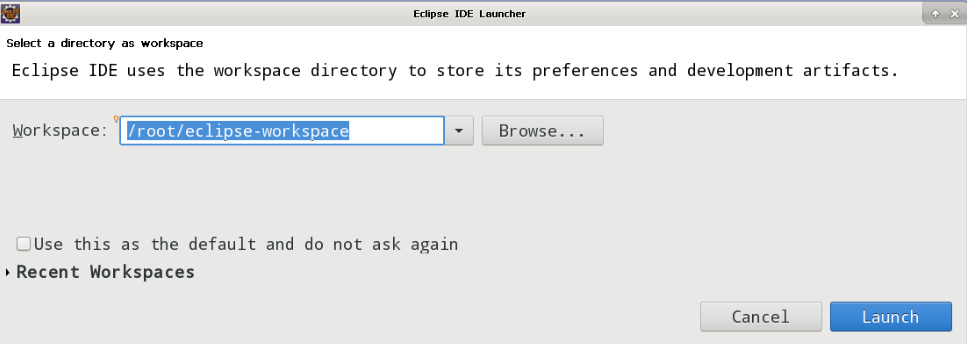
\includegraphics[width=4.5in]{figures/fig1.png}
					\end{figure}
					\begin{figure}[H]
						\centering
						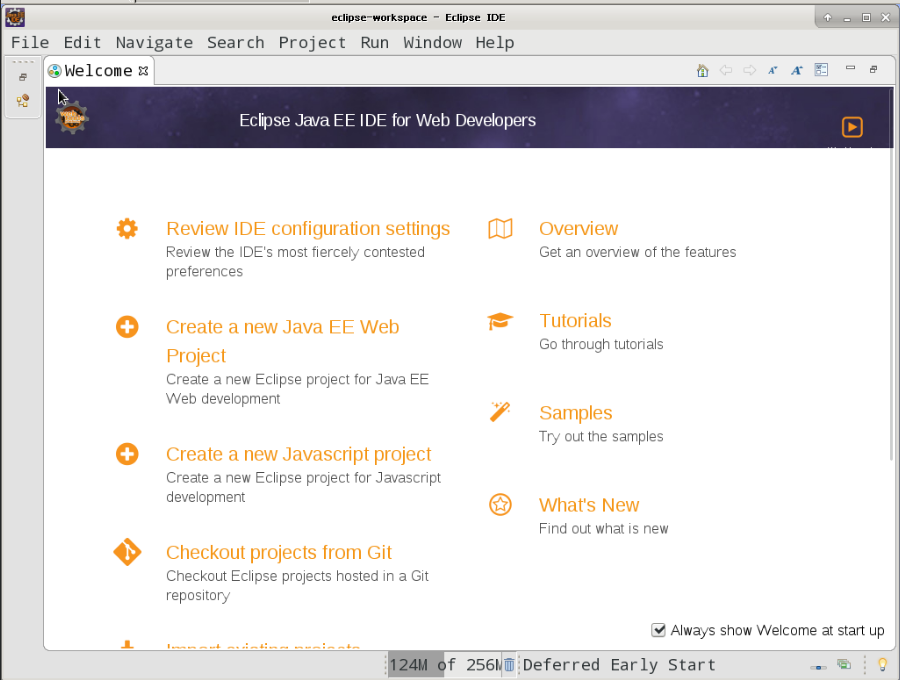
\includegraphics[width=4.5in]{figures/fig2.png}
					\end{figure}
				
					\item 关闭Welcome页面。
					\begin{figure}[H]
						\centering
						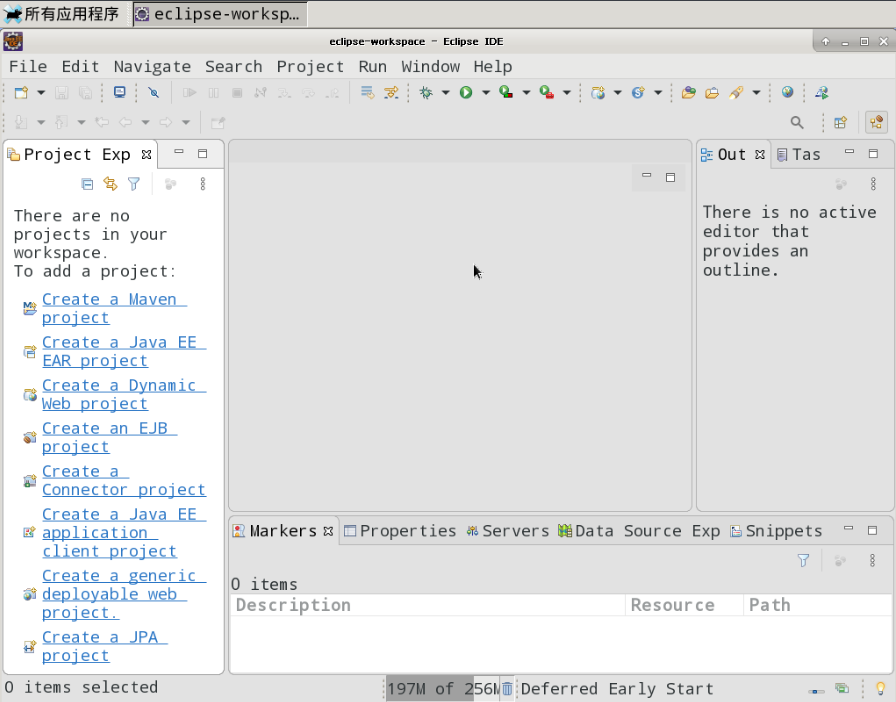
\includegraphics[width=4.5in]{figures/fig3.png}
					\end{figure}
				
					\item 点击Window->Preferences,左侧对话框选择Hadoop Map/Reduce选项。
					\begin{figure}[H]
						\centering
						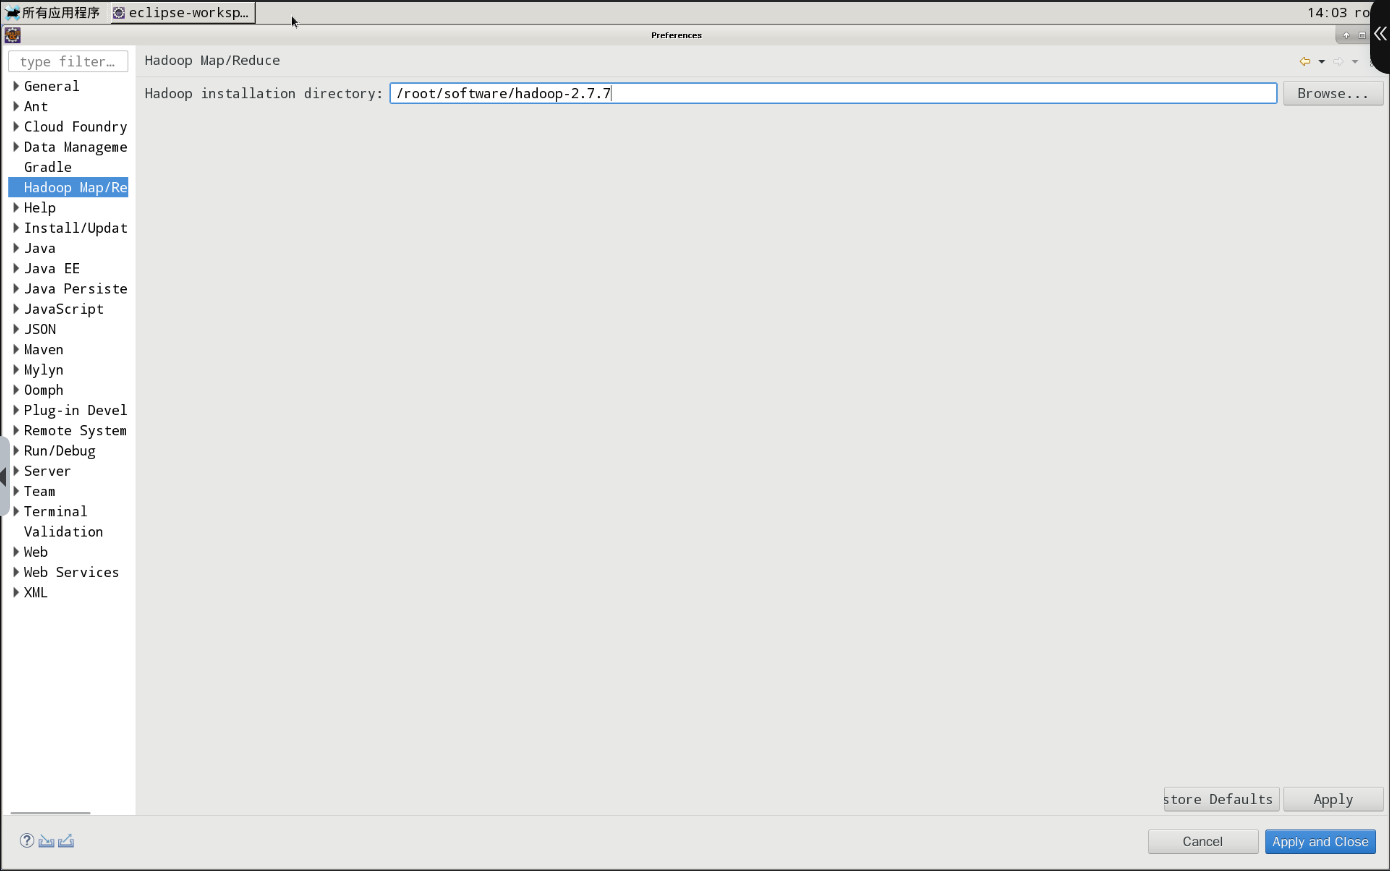
\includegraphics[width=4.5in]{figures/fig4.png}
					\end{figure}
				
					\item 设置hadoop-2.7.7的安装路径。(实验环境hadoop-2.7.7的安装目录为:/root/software/hadoop-2.7.7)。
					\begin{figure}[H]
						\centering
						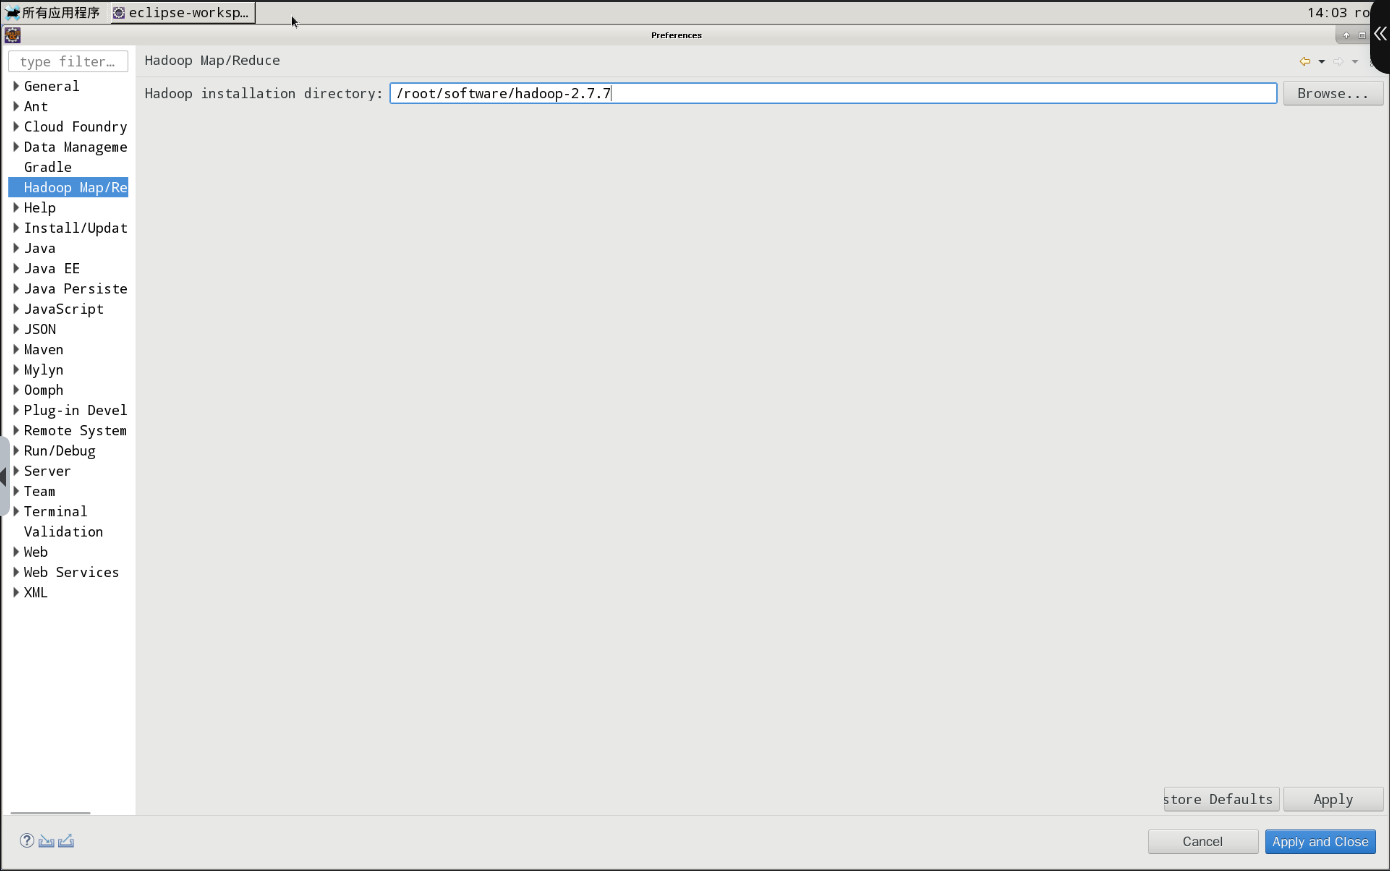
\includegraphics[width=4.5in]{figures/fig4.png}
					\end{figure}
				
					\item 点击Apply and Close。
					\item 点击Window->Show View->Other,弹出Show View对话框,选中MapReduce Tools下的Map/Reduce Locations,点击Open。
					\begin{figure}[H]
						\centering
						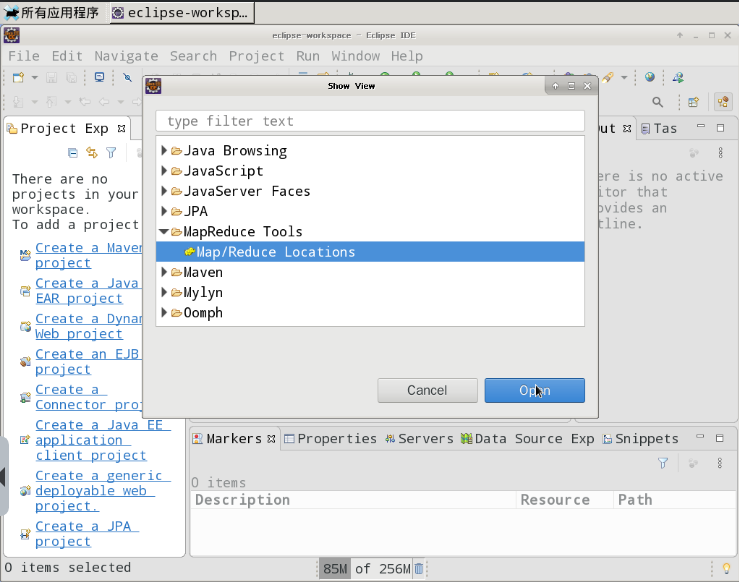
\includegraphics[width=4in]{figures/fig5.png}
					\end{figure}
				
					\item Eclipse底部出现Map/Reduce Locations窗口,点击其右边的蓝色小象图标。
					\begin{figure}[H]
						\centering
						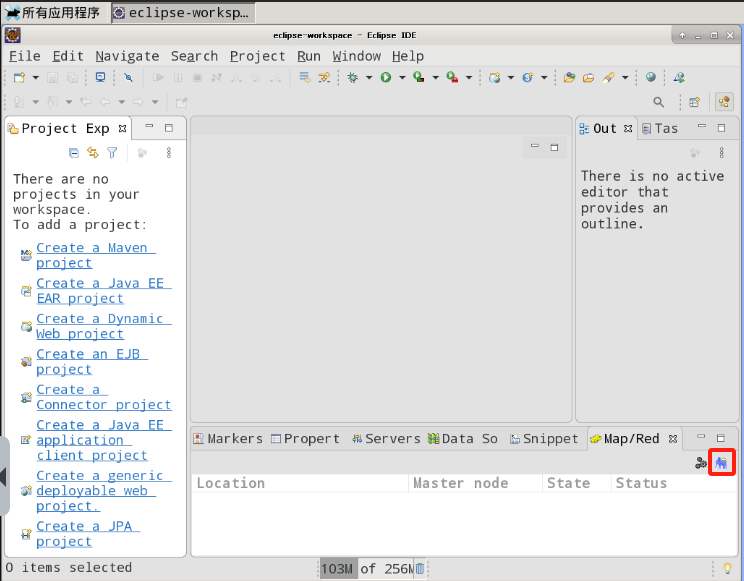
\includegraphics[width=4in]{figures/fig6.png}
					\end{figure}
				
					\item 弹出New Hadoop locaiton...对话框,将Location name命名为hadoop。
					\begin{figure}[H]
						\centering
						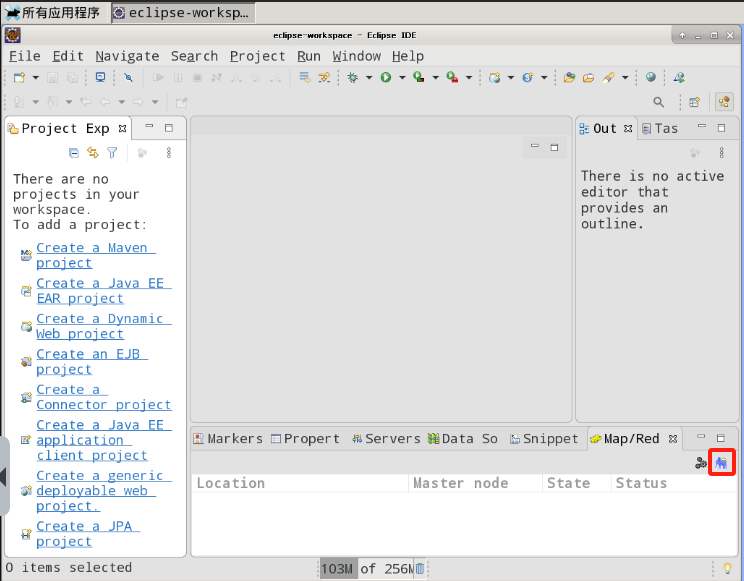
\includegraphics[width=4in]{figures/fig6.png}
					\end{figure}
				
					\item Map/Reduce(V2)Master下将Host修改为YARN集群主节点的IP地址或主机名localhost。
					\item DFS Master下将Host修改为HDFS集群主节点的IP地址或主机名localhost,Port修改为9000,将User name设置为搭建集群用户root。
					\begin{figure}[H]
						\centering
						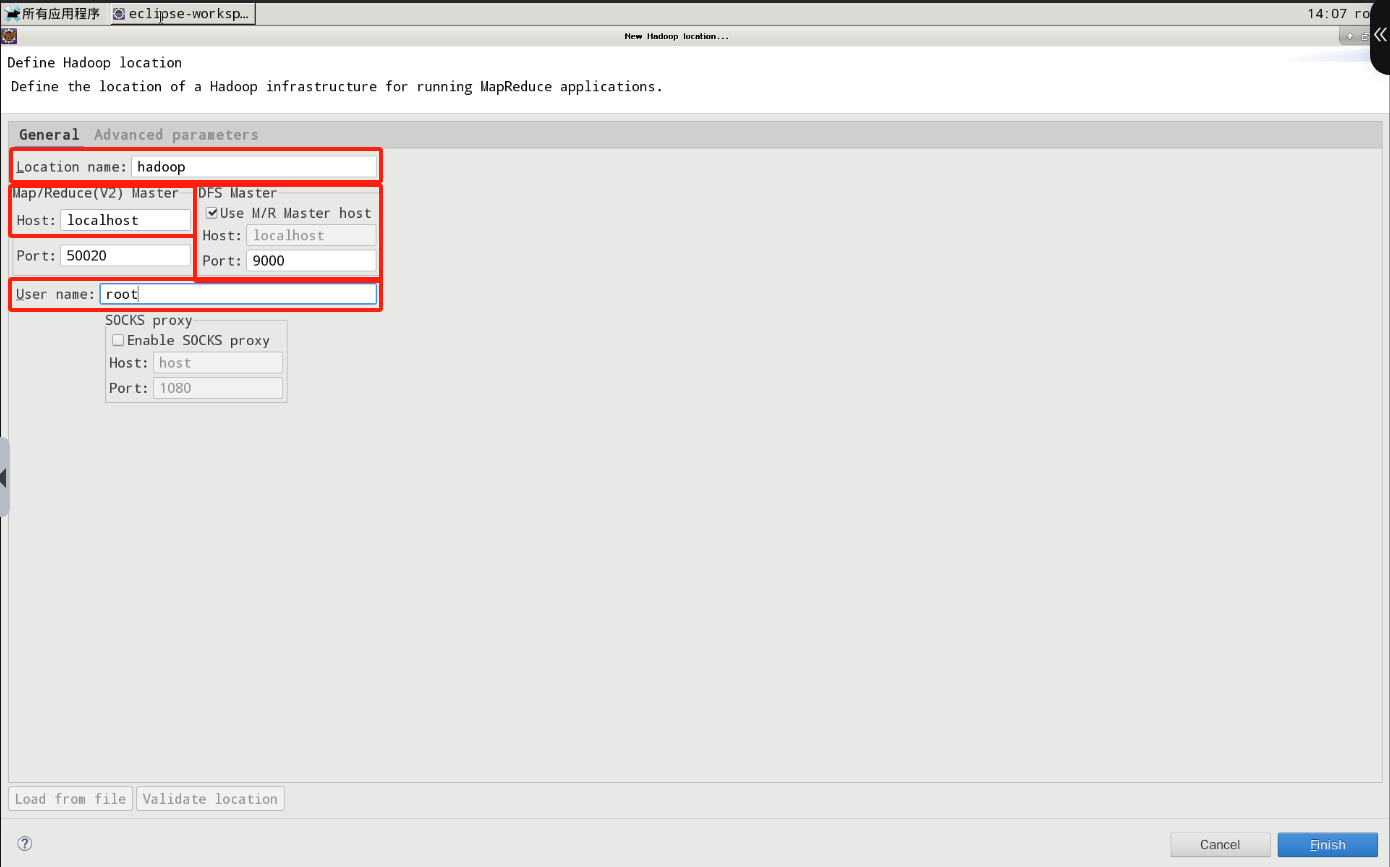
\includegraphics[width=3.5in]{figures/fig7.png}
					\end{figure}
				\end{enumerate}
			
				测试连接:
				\begin{enumerate}
					\item 选择File->New->Project->Map/Reduce Project->Next,弹出new MapReduce Project Wizard对话框。
					\begin{figure}[H]
						\centering
						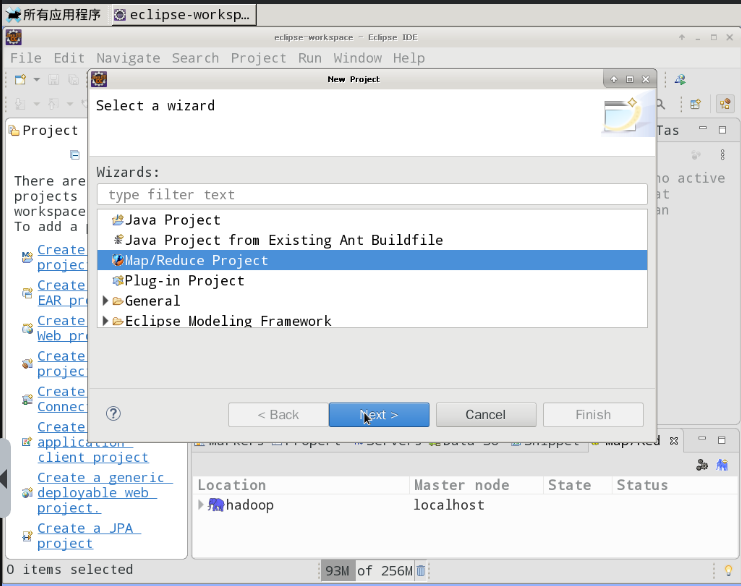
\includegraphics[width=3.5in]{figures/fig8.png}
					\end{figure}
				
					\item 为Project name起名为Test,点击Finsh。
					\begin{figure}[H]
						\centering
						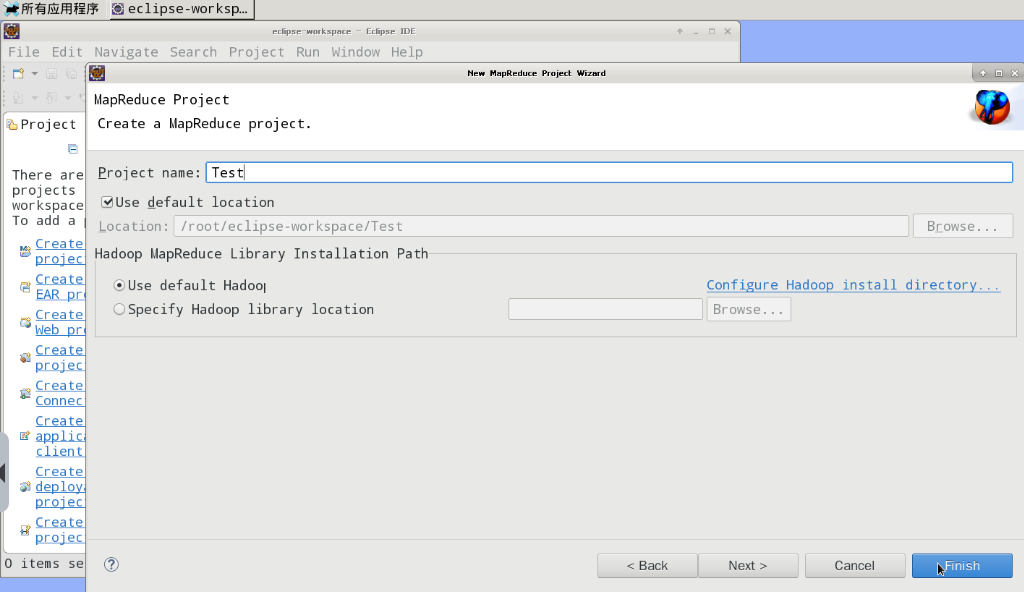
\includegraphics[width=4.5in]{figures/fig9.png}
					\end{figure}
				
					\item 弹出Open Associated Perspective对话框选择No。
					\begin{figure}[H]
						\centering
						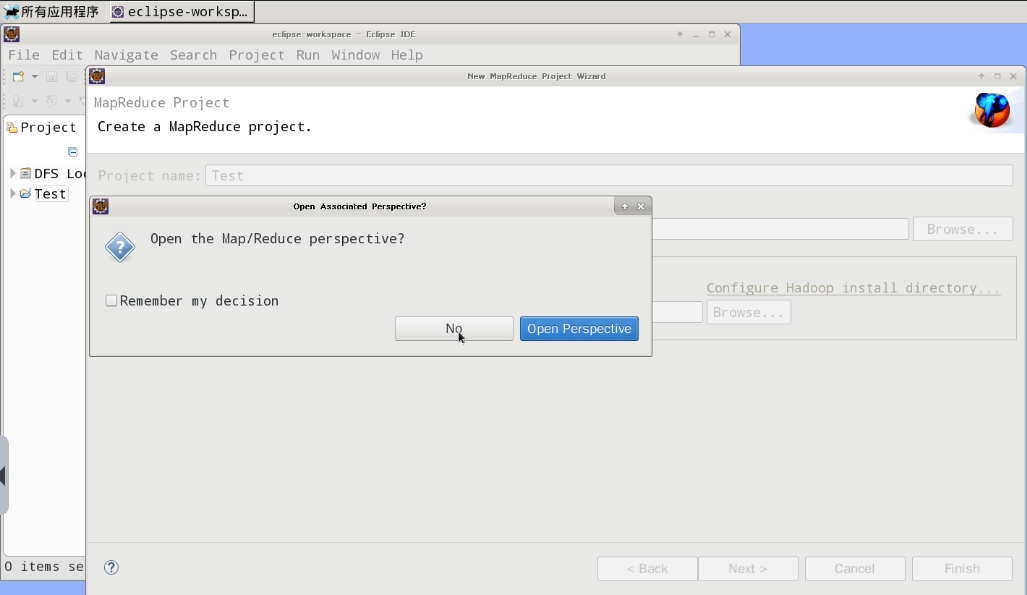
\includegraphics[width=4.5in]{figures/fig10.png}
					\end{figure}
				
					\item 在左侧Project Explorer下出现DFS Locations列表栏和Test。
					\begin{figure}[H]
						\centering
						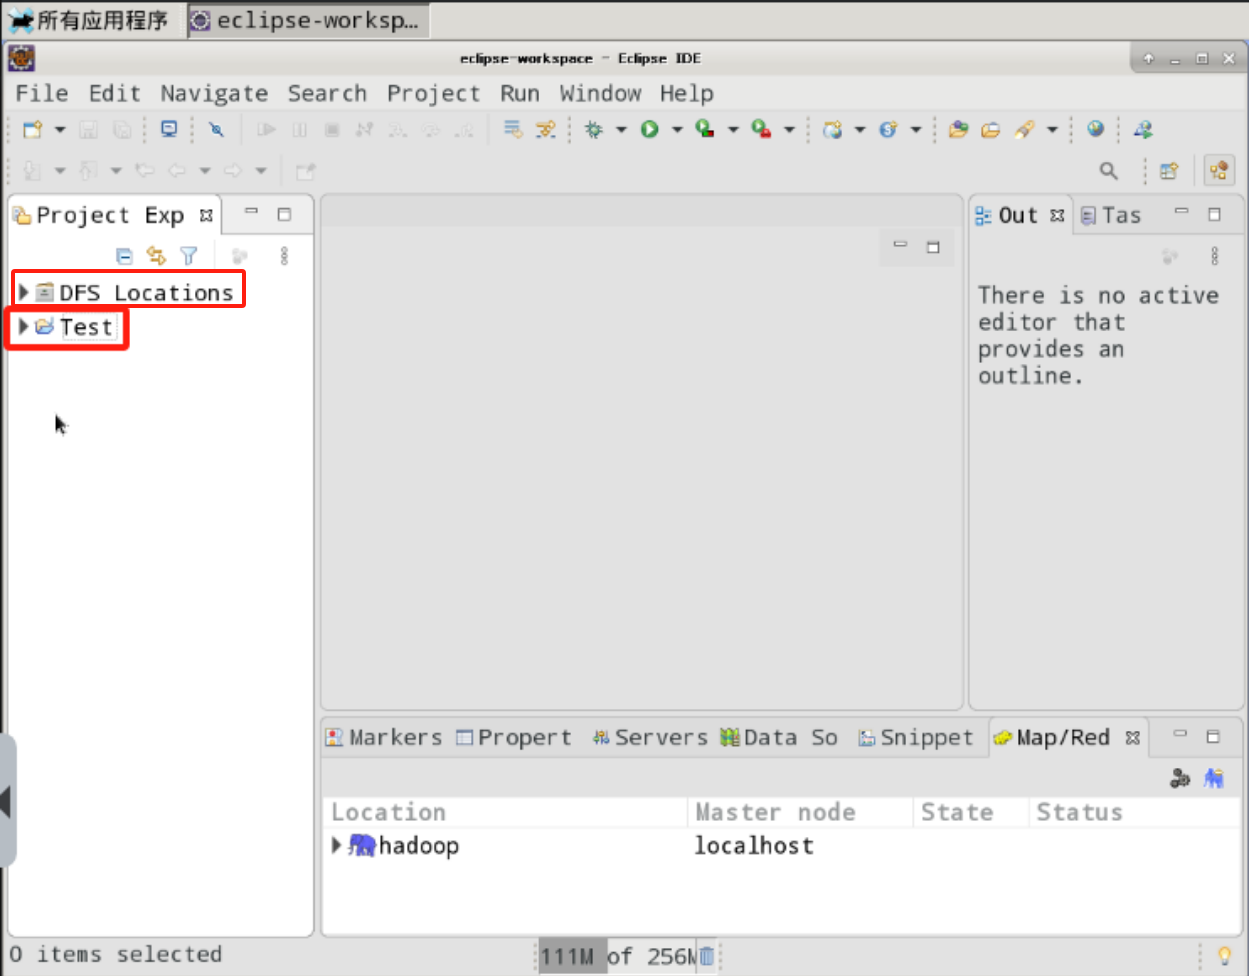
\includegraphics[width=3.5in]{figures/fig11.jpg}
					\end{figure}
				\end{enumerate}
				
				至此,Hadoop已经可以连接上Eclipse。后续可进行程序开发。
				
			\subsubsection{获取FileSystem实例演示}
				创建项目:
				\begin{enumerate}
					\item 选择File->New->Project->Map/Reduce Project->Next,弹出new MapReduce Project Wizard对话框。Project name命名为:getFS,点击Finsh
					\begin{figure}[H]
						\centering
						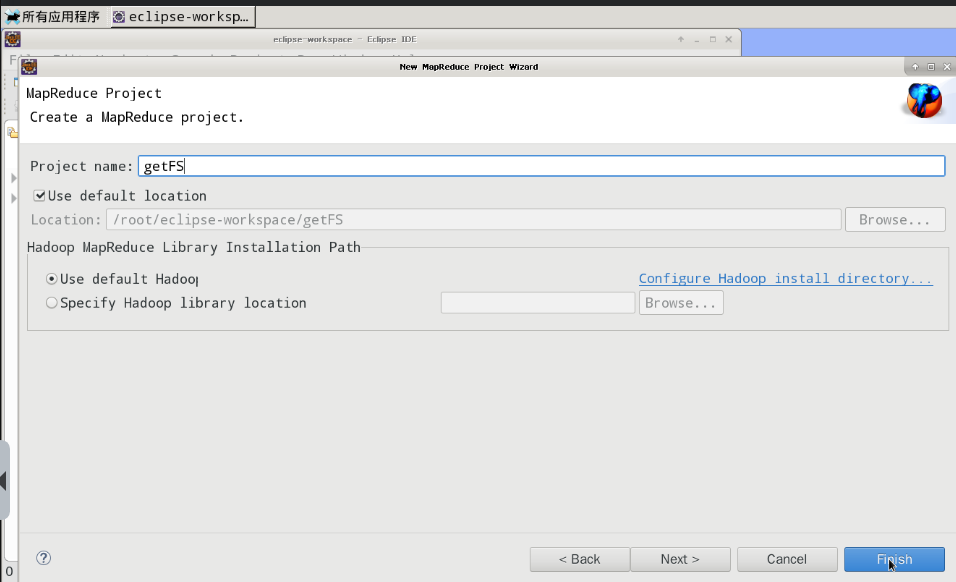
\includegraphics[width=4.5in]{figures/fig12.png}
					\end{figure}
				
					\item 点击左侧getFS,在src下创建包结构:com.hongya.getfs。
					\begin{figure}[H]
						\centering
						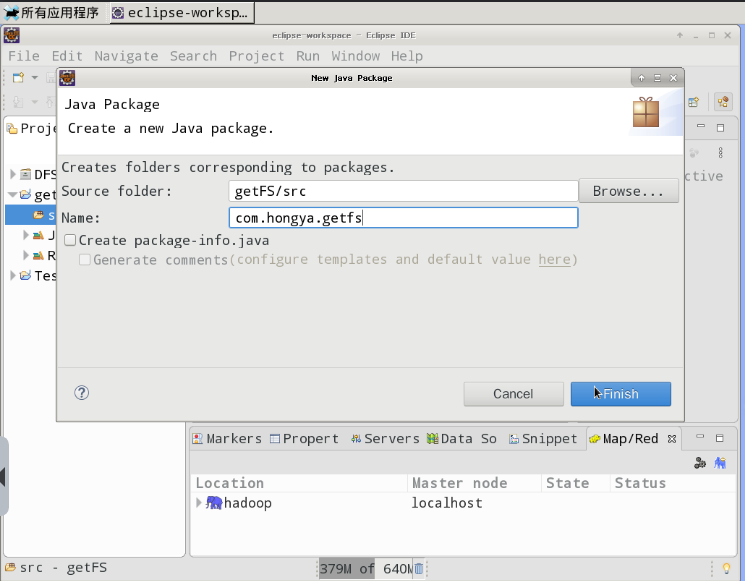
\includegraphics[width=4in]{figures/fig13.png}
					\end{figure}
				
					\item 在包下创建测试类Test1,Test2。
					\begin{figure}[H]
						\centering
						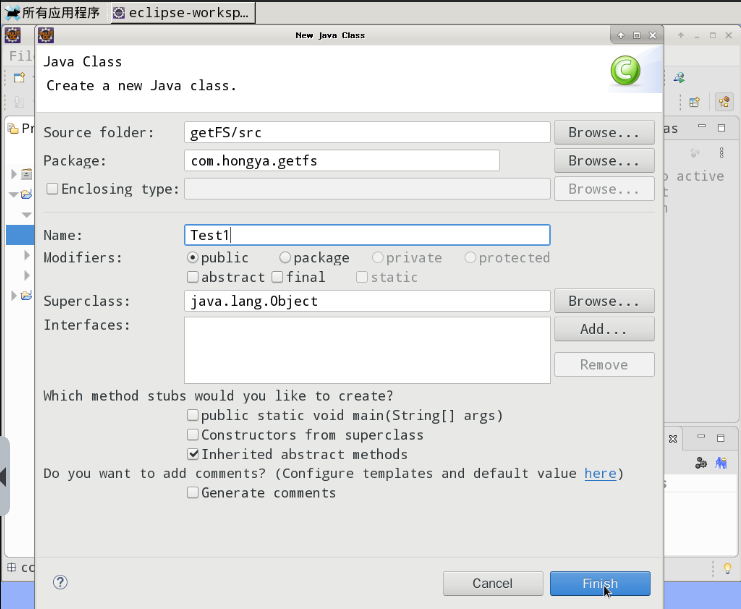
\includegraphics[width=4in]{figures/fig14.png}
					\end{figure}
					\begin{figure}[H]
						\centering
						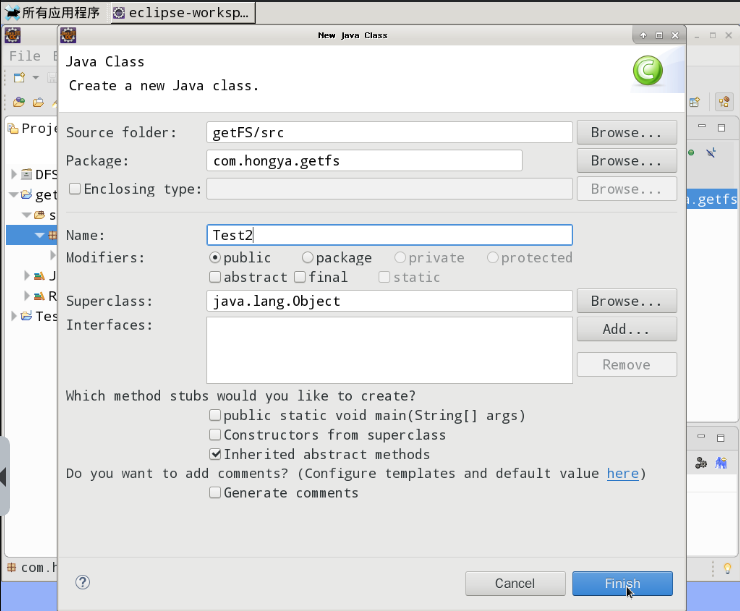
\includegraphics[width=4in]{figures/fig15.png}
					\end{figure}
				\end{enumerate}
			
				通过配置获取FileSystem对象:
				\begin{enumerate}
					\item 在Test1下使用new构造Configuration对象,获取配置信息类。
					\item 通过set方法设置配置项,指定文件系统为HDFS,即fs.defaultFS参数的值为hdfs://localhost:9000。
					\item 获取文件系统对象并打印URI地址。
					\begin{figure}[H]
						\centering
						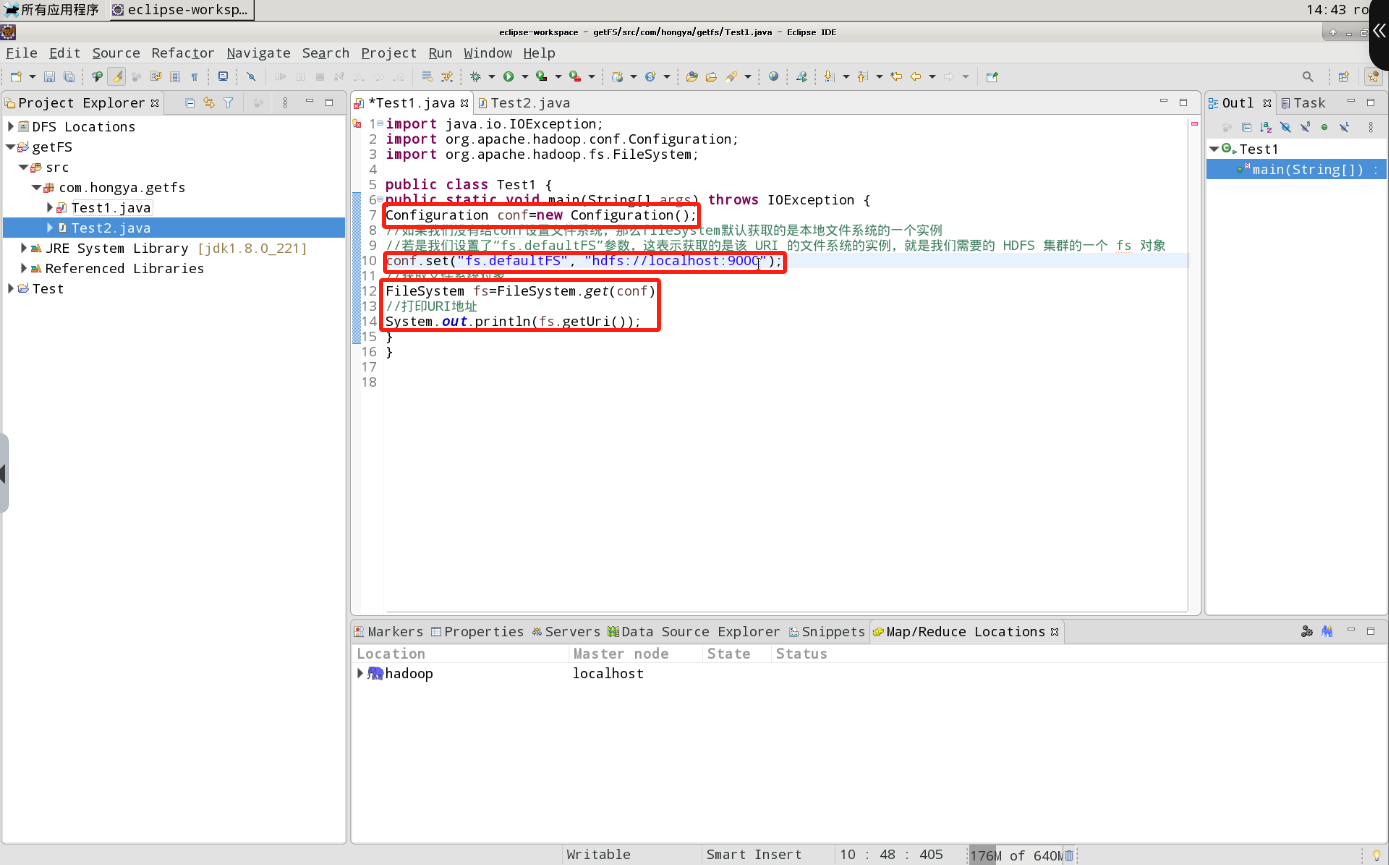
\includegraphics[width=4in]{figures/fig16.png}
					\end{figure}
				\end{enumerate}
			
				直接获取FileSystem对象:
				\begin{enumerate}
					\item 在Test2中用new构造Configuration对象,获取配置信息类。
					\item 通过get方法获取HDFS文件系统对象,设置URI为hdfs://localhost:9000,安装集群用户名为root。
					\item 打印获取的文件系统URI。
					\begin{figure}[H]
						\centering
						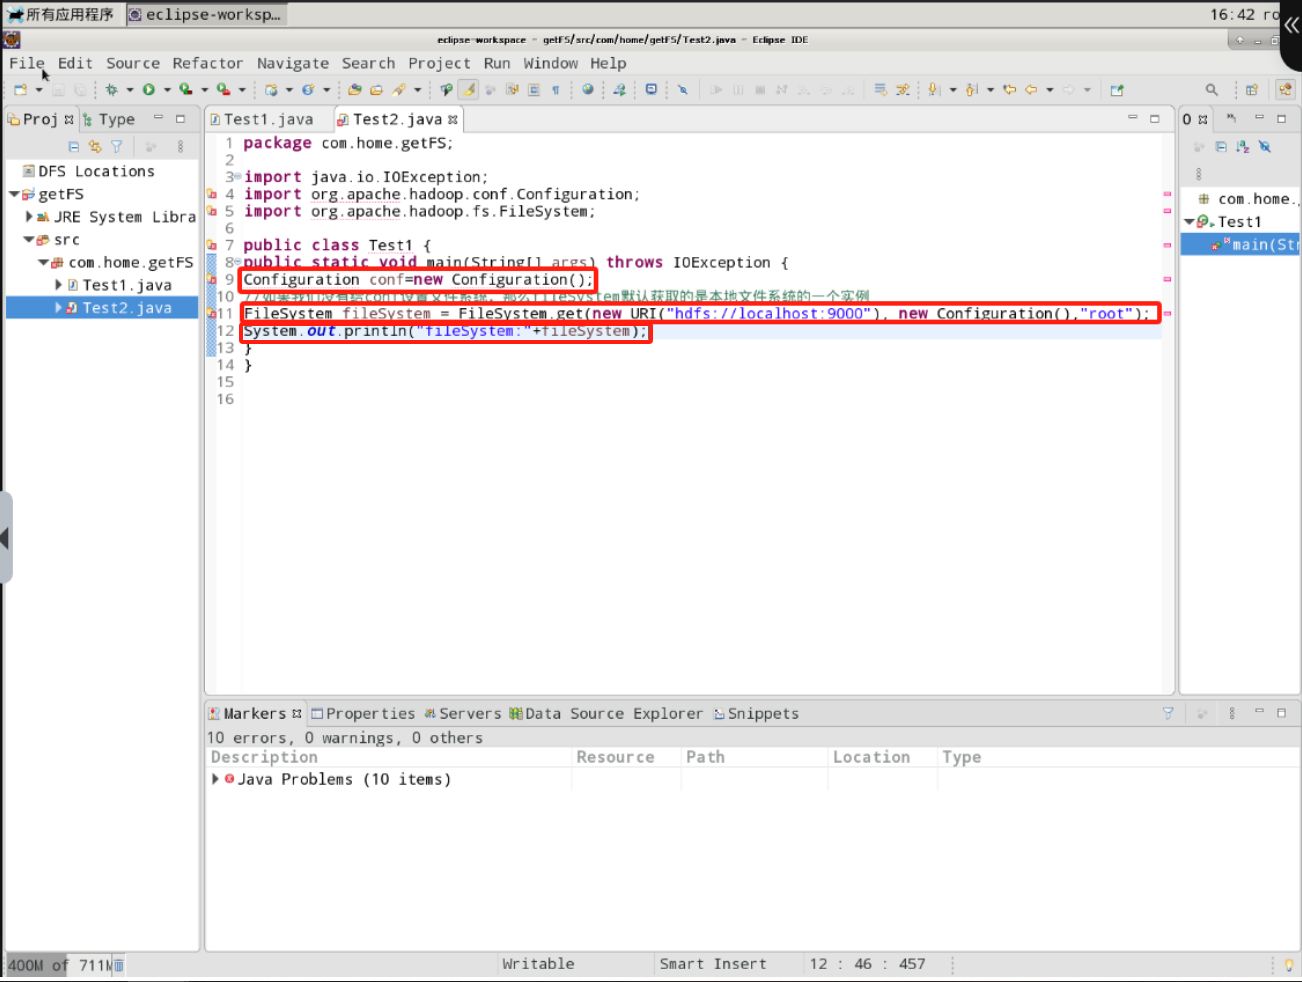
\includegraphics[width=4.5in]{figures/fig16.5.png}
					\end{figure}
				\end{enumerate}
			
		\subsection{上传查看文件操作}
			\subsubsection{创建目录}
				创建项目:
				\begin{enumerate}
					\item 项目名:Api\_hdfs。
					\item 包名:com.hongya.api\_hdfs 。
					\item 类:
					\begin{itemize}
						\item 创建目录类:MkDemo。
						\item 上传文件类:PutDemo。
						\item 遍历文件类:ListDemo。
					\end{itemize}
					\begin{figure}[H]
						\centering
						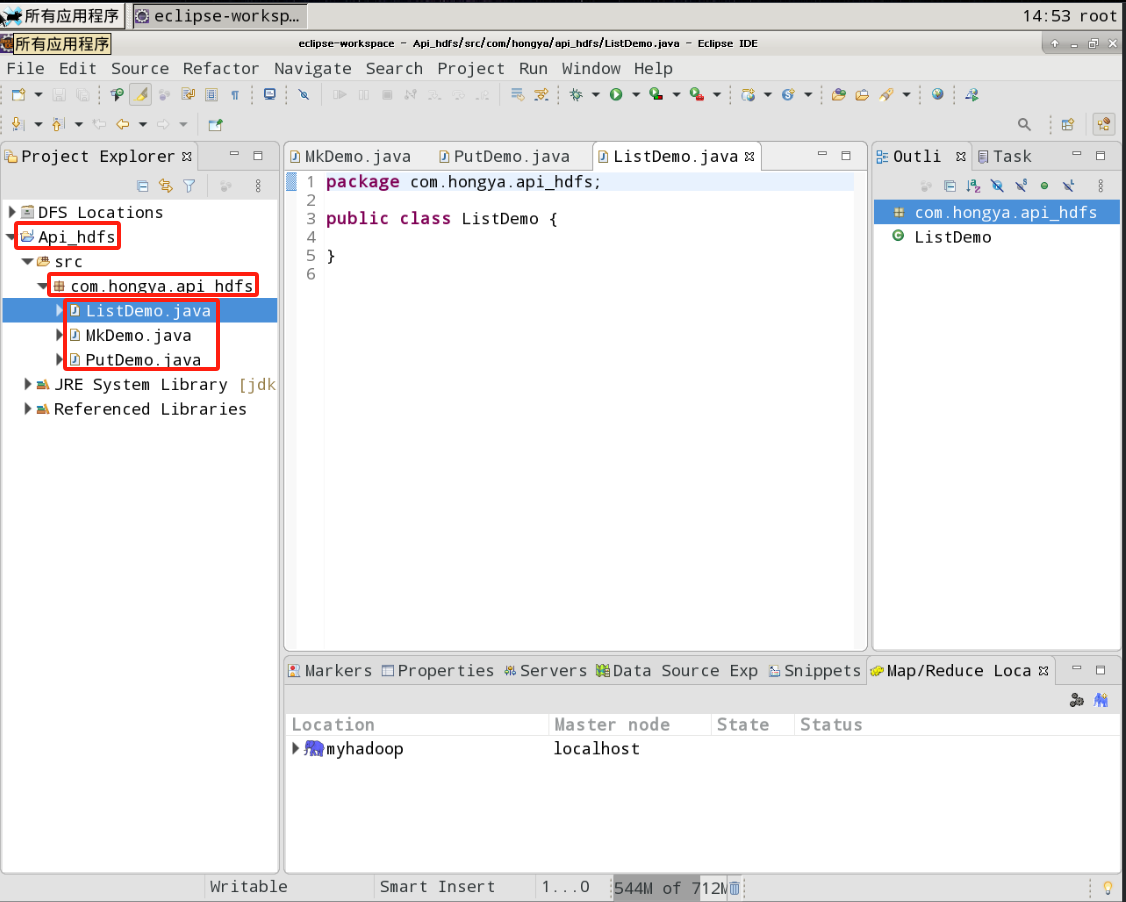
\includegraphics[width=4.5in]{figures/fig17.png}
					\end{figure}
				\end{enumerate}
			
				代码逻辑:
				\begin{enumerate}
					\item 在MkDemo类中使用单元测试方法。
					\item 直接创建FileSystem对象。
					\item 使用mkdirs方法在根目录下创建test文件夹。
					\item 关闭资源。
					\item 运行程序并在Eclipse中的DFS Locations列表栏查看文件夹创建是否成功。
					\begin{figure}[H]
						\centering
						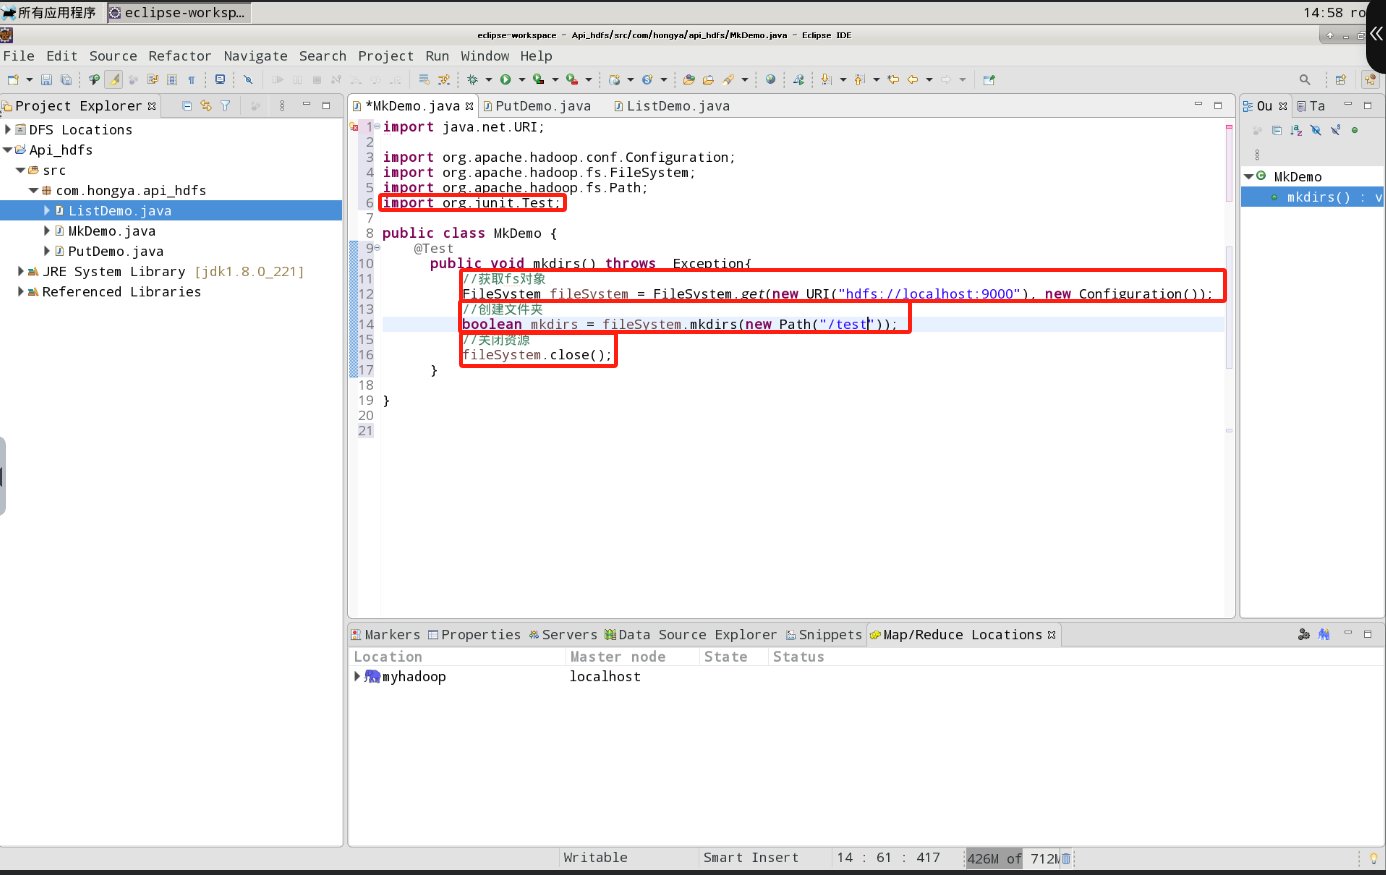
\includegraphics[width=4.5in]{figures/fig18.png}
					\end{figure}
				\end{enumerate}
			
			\subsubsection{任务2:上传文件}
				在本地/root目录下创建test.txt文件。添加如下内容:\\
				HDFS\_API
				
				\begin{figure}[H]
					\centering
					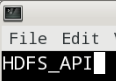
\includegraphics{figures/fig19.png}
				\end{figure}
				
				代码逻辑:
				\begin{enumerate}
					\item 在PutDemo类中使用单元测试方法。
					\item 创建FileSystem对象。
					\item 使用copyFromLocalFile方法上传文件test.txt。
					\item 关闭资源。
					\item 运行程序并在Eclipse中的DFS Locations列表栏查看文件上传是否成功。
					\begin{figure}[H]
						\centering
						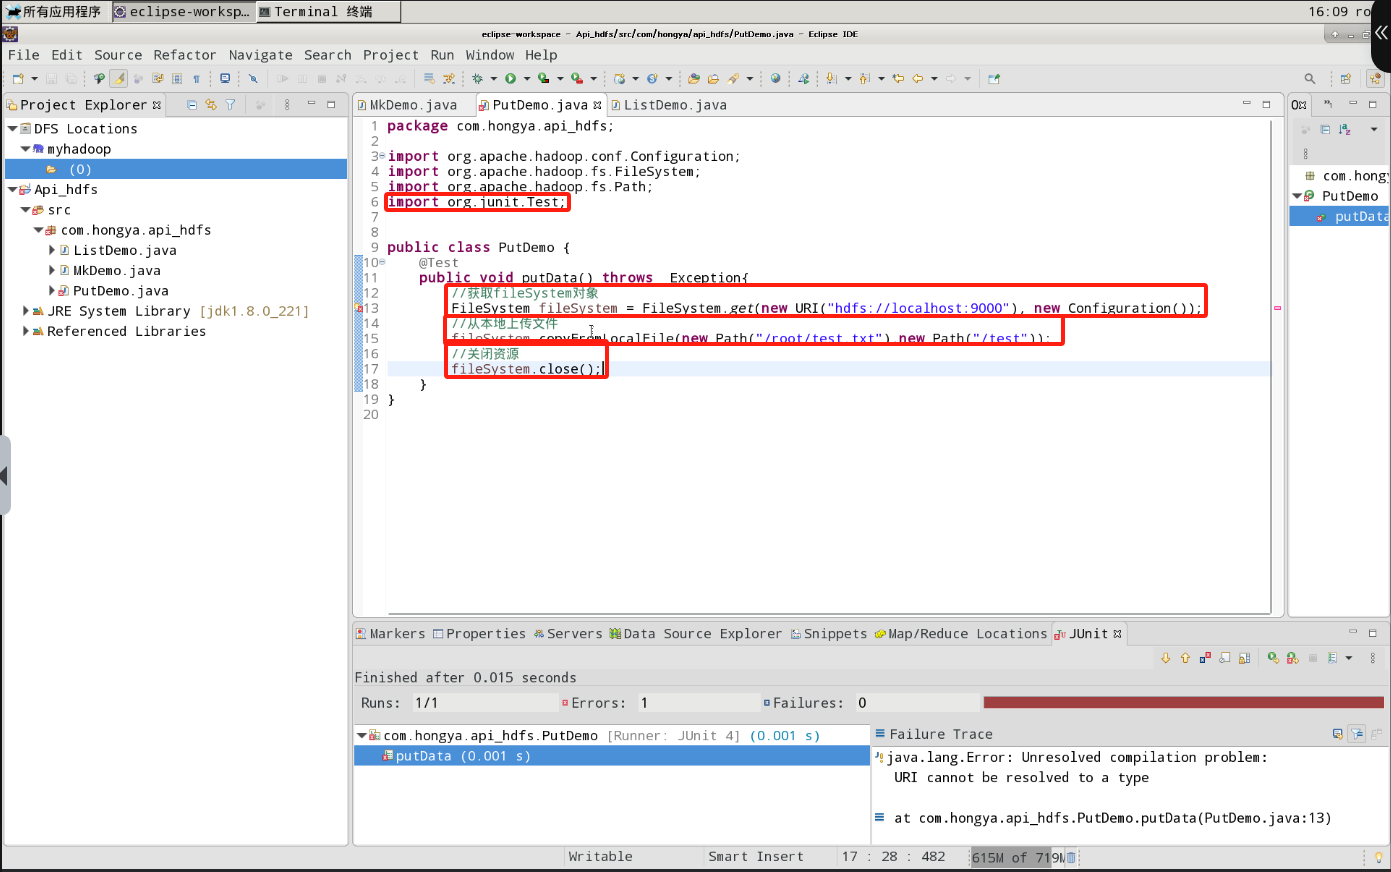
\includegraphics[width=4in]{figures/fig20.png}
					\end{figure}
				\end{enumerate}
			
			\subsubsection{任务3:遍历文件}
				遍历文件代码逻辑:
				\begin{enumerate}
					\item 在ListDemo类中使用单元测试方法。
					\item 获取FileSystem对象。
					\item 通过listFiles方法获取RemoteIterator得到所有的文件或者文件夹。
					\item 递归遍历并打印文件夹或文件路径。
					\item 关闭资源。
					\begin{figure}[H]
						\centering
						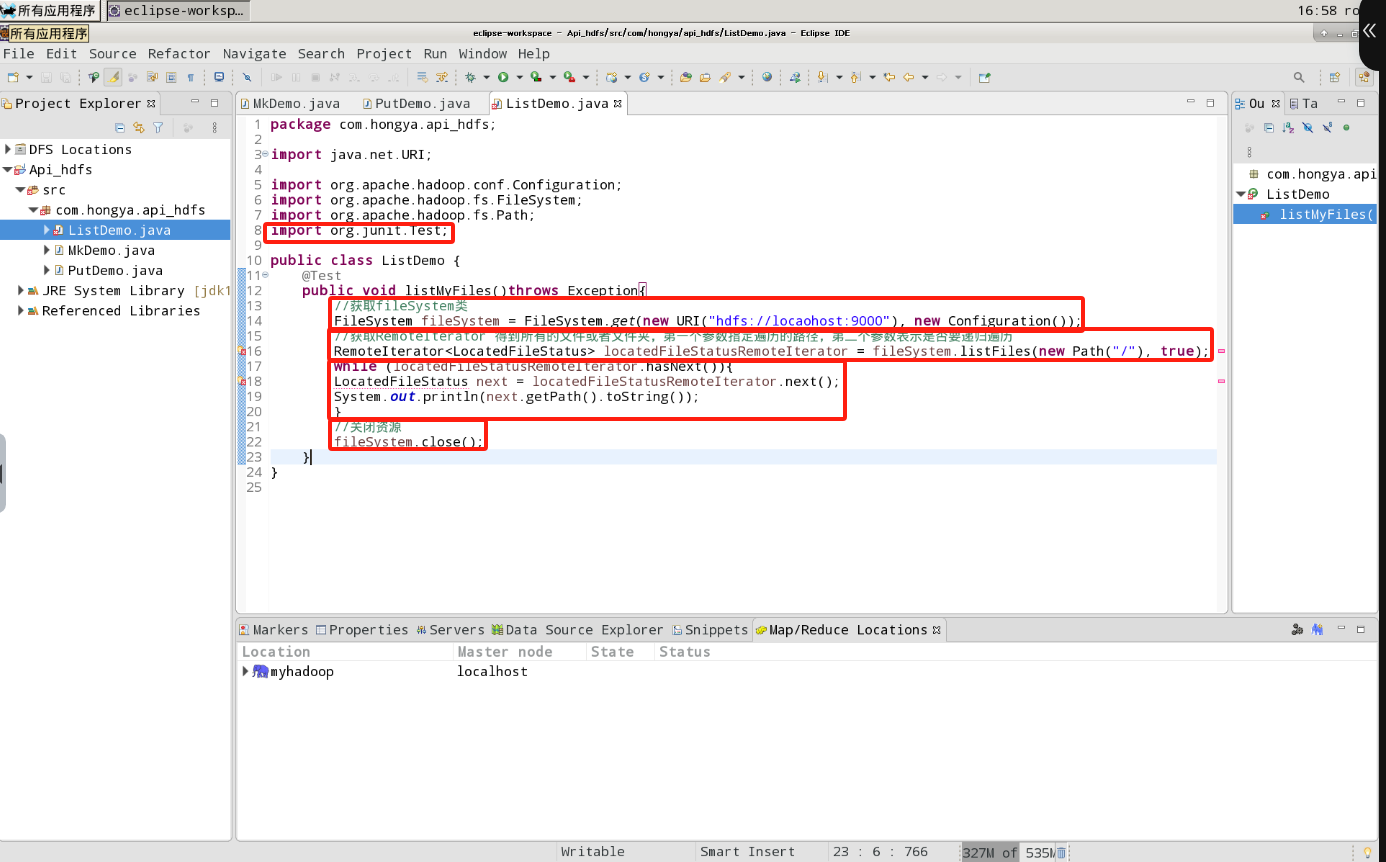
\includegraphics[width=4in]{figures/fig20.5.jpg}
					\end{figure}
					\item 运行程序查看控制台输出。
				\end{enumerate}
			
		\subsection{修改删除文件操作}
			\subsubsection{下载文件}
				创建项目:
				\begin{enumerate}
					\item 项目名:Api\_hdfs。
					\item 包名:com.hongya.api\_hdfs 。
					\item 类:
					\begin{itemize}
						\item 下载文件类:GetDemo。
						\item 重命名目录文件类:ReDemo。
						\item 重命名目录文件类:ReDemo。
					\end{itemize}
					\begin{figure}[H]
						\centering
						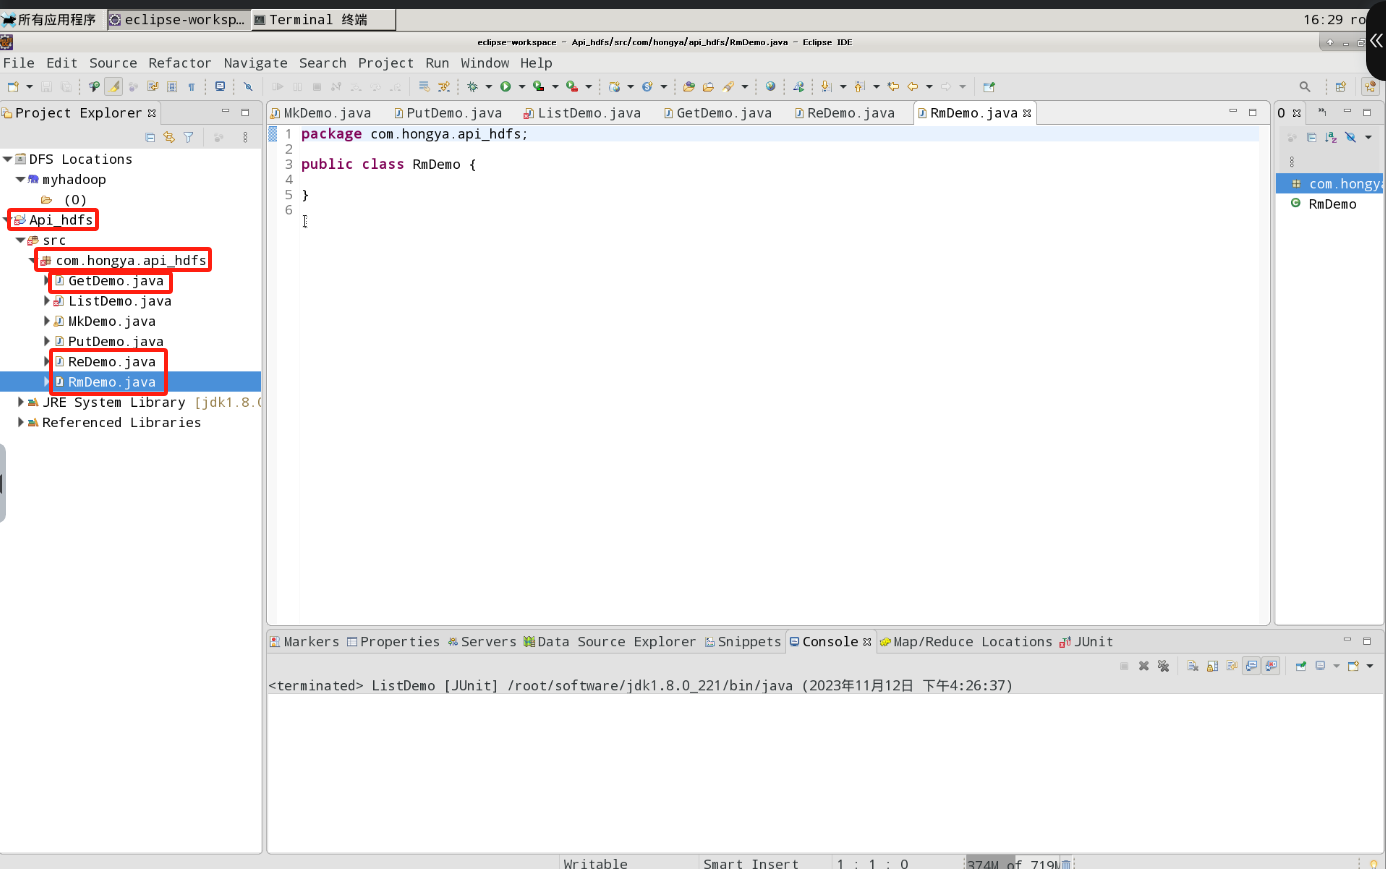
\includegraphics[width=4.5in]{figures/fig21.png}
					\end{figure}
				\end{enumerate}
			
				数据准备:	
				\begin{enumerate}
					\item 在本地/目录下创建test.txt文件,添加内容如下:\\
					copyTolocalfile() \\
					rename() \\
					delete()
					
					\begin{figure}[H]
						\centering
						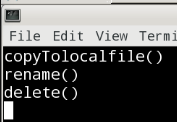
\includegraphics{figures/fig22.png}
					\end{figure}
				
					\item 创建并上传test.txt文件到HDFS目录:/test \\
					需求:将HDFS文件test.txt下载到本地/root目录。
					\begin{figure}[H]
						\centering
						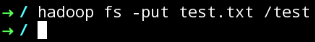
\includegraphics{figures/fig21.5.png}
					\end{figure}
				\end{enumerate}
			
				下载文件代码逻辑:
				\begin{enumerate}
					\item 在GetDemo类中使用单元测试方法。
					\item 直接创建FileSystem对象。
					\item 使用copyTolocalfile方法将test.txt文件下载到/root。
					\item 关闭资源。
					\begin{figure}[H]
						\centering
						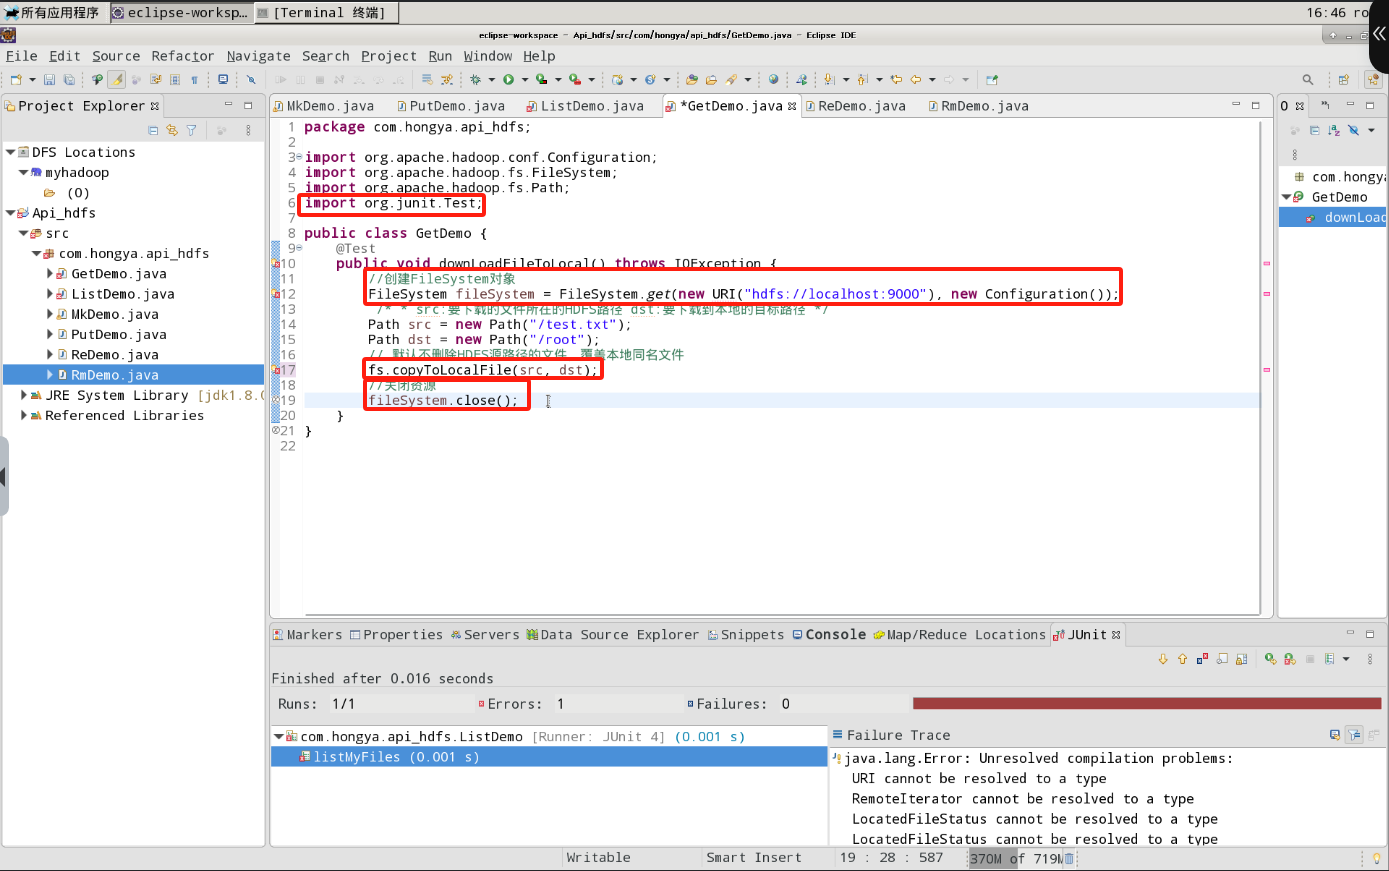
\includegraphics[width=4.5in]{figures/fig23.png}
					\end{figure}
				\end{enumerate}
				
				查看结果:进入/root目录通过ls或ll命令查看test.txt文件是否成功下载。
				
			\subsubsection{任务2:重命名目录文件}
				需求1:将test.txt文件重命名为tmp.txt。\\
				需求2:将test文件夹重命名为tmp。
				
				代码逻辑:
				\begin{enumerate}
					\item 在ReDemo类中使用单元测试方法。
					\item 直接创建FileSystem对象。
					\item 使用rename方法重命名目录文件。
					\item 关闭资源。
					\begin{figure}[H]
						\centering
						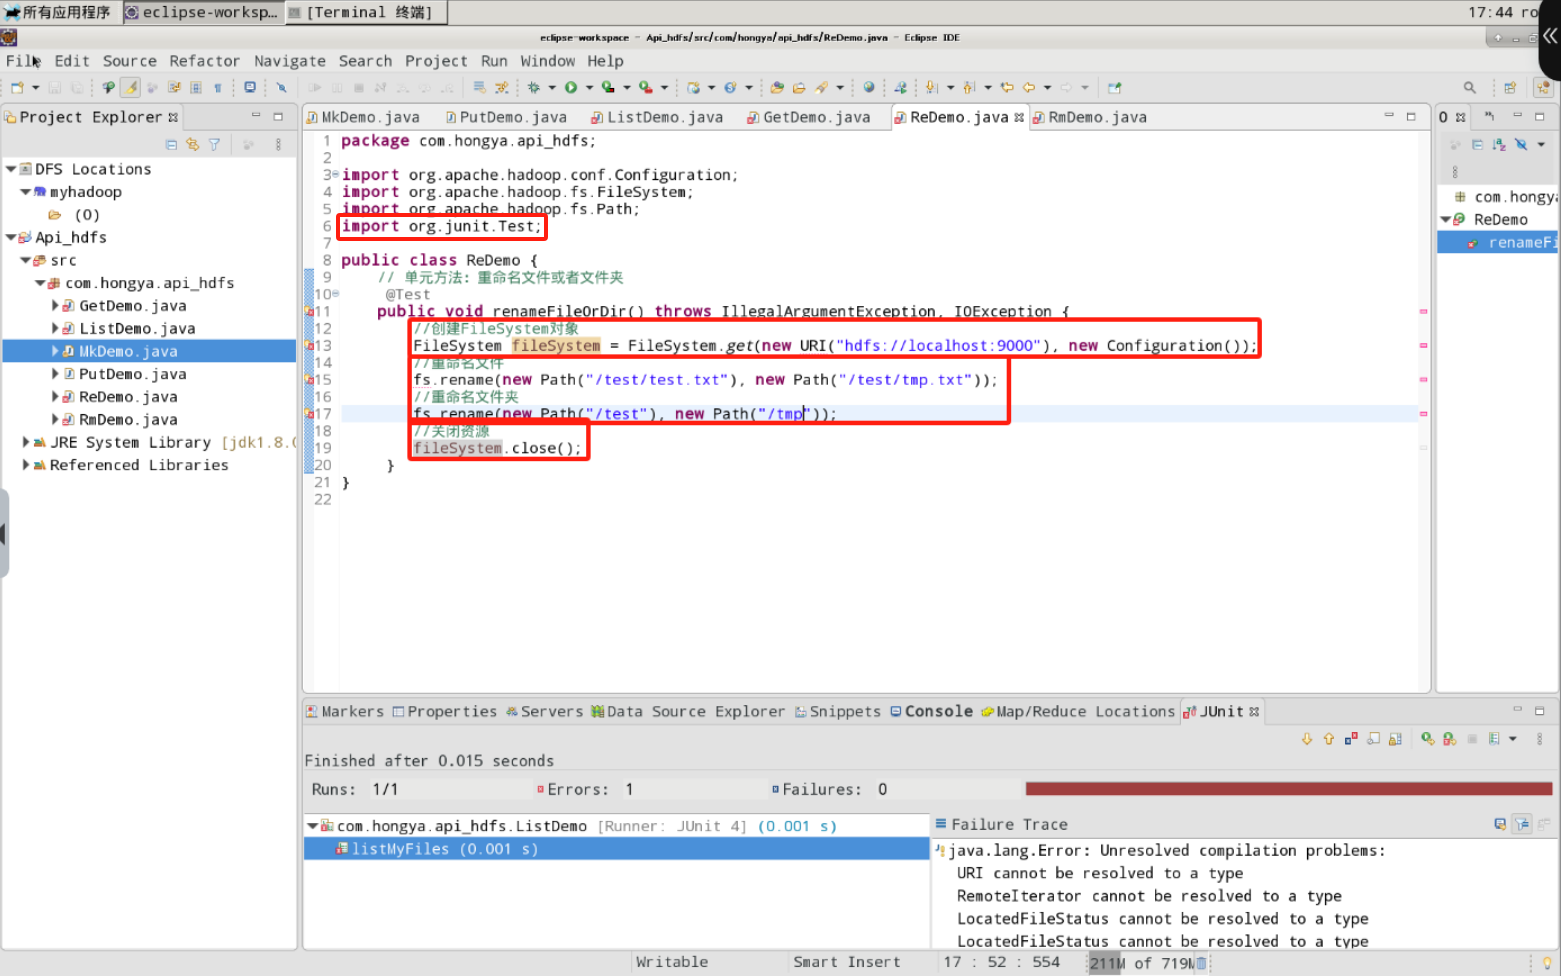
\includegraphics[width=4.5in]{figures/fig24.png}
					\end{figure}
				\end{enumerate}
			
			\subsubsection{任务3:删除目录文件}
				需求1:删除任务二中修改后文件tmp.txt。\\
				需求2:删除任务二中修改后文件夹tmp。
				
				代码逻辑:
				\begin{enumerate}
					\item 在RmDemo类中使用单元测试方法。
					\item 直接创建FileSystem对象。
					\item 使用delete方法删除目录文件。
					\item 关闭资源。
					\item 运行程序并在Eclipse中的DFS Locations列表栏查看目录文件删除是否成功。
					\begin{figure}[H]
						\centering
						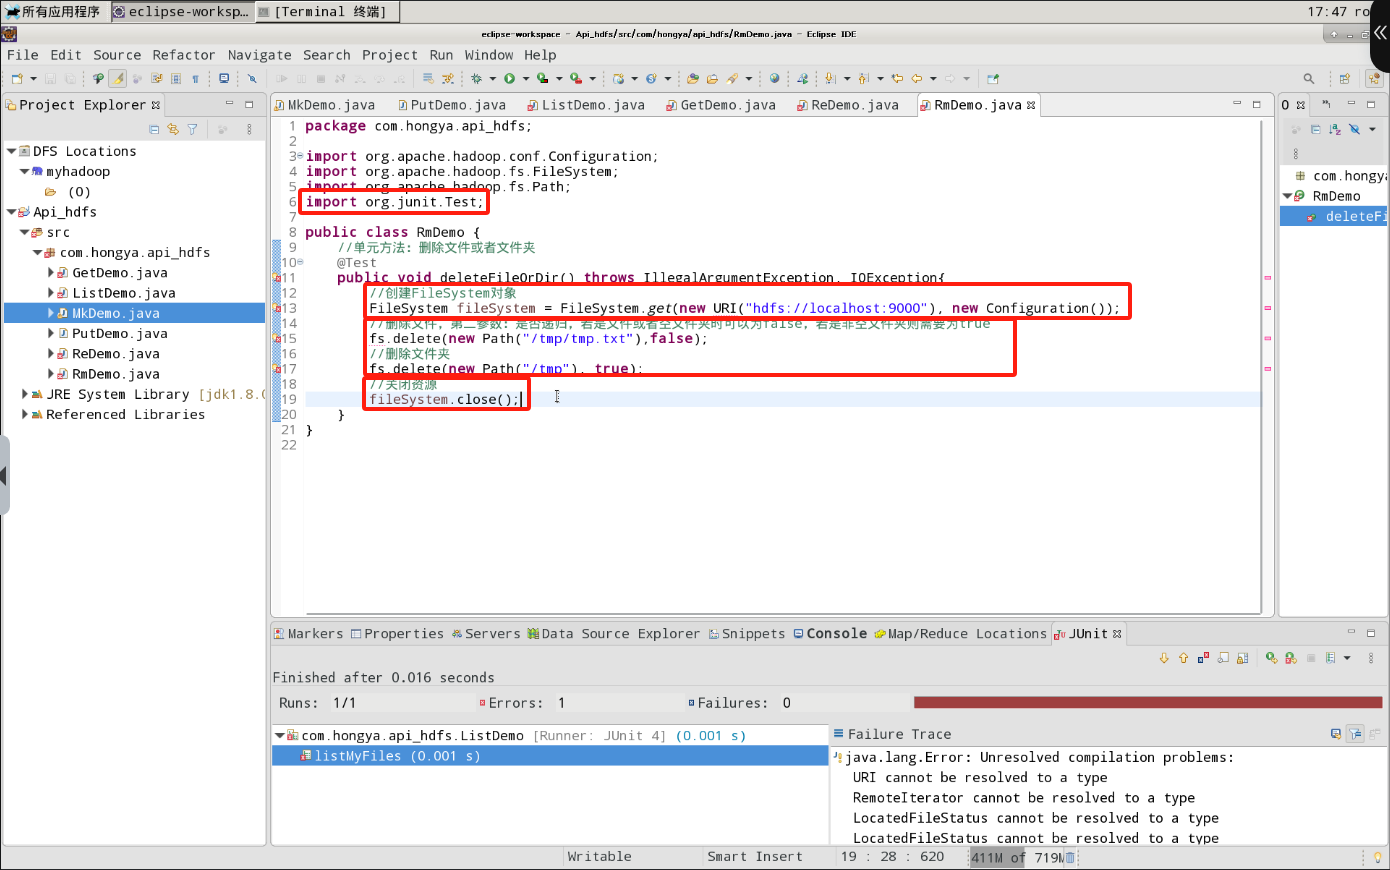
\includegraphics[width=3.5in]{figures/fig25.png}
					\end{figure}
				\end{enumerate}
			
			\subsubsection{小文件合并}
				任务:合并小文件操作
				
				创建项目:
				\begin{enumerate}
					\item 项目名:Api\_hdfs。
					\item 包结构:com.hongya.api\_hdfs。
					\item 合并文件实现类:MergeDemo。
					\begin{figure}[H]
						\centering
						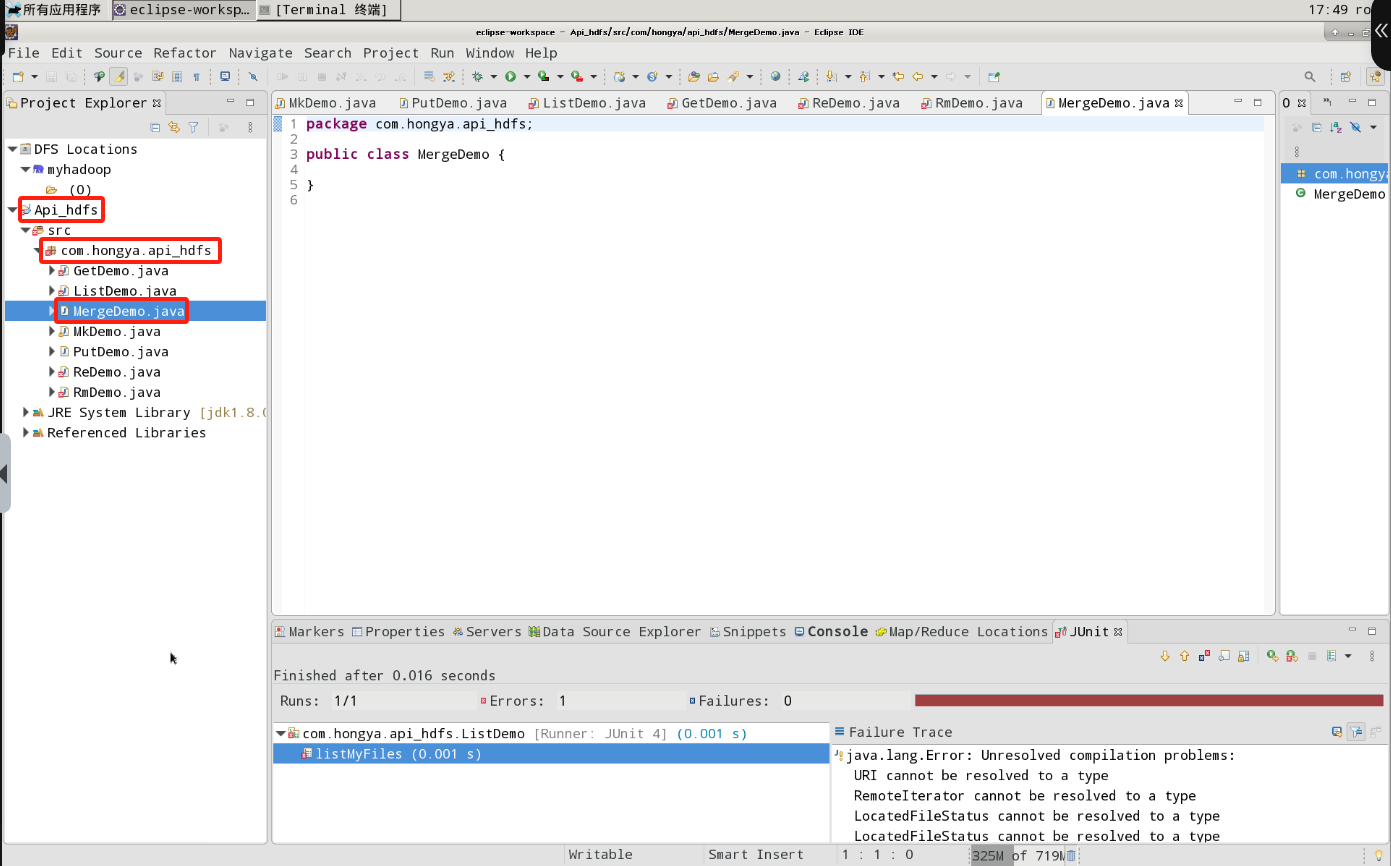
\includegraphics[width=3.5in]{figures/fig26.png}
					\end{figure}
				\end{enumerate}
			
				数据准备:
				\begin{enumerate}
					\item 在本地/root目录下创建目录input。
					\begin{figure}[H]
						\centering
						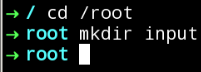
\includegraphics{figures/fig27.png}
					\end{figure}
				
					\item 在input目录下创建a.txt文件,添加如下内容:\\
					123
					
					\begin{figure}[H]
						\centering
						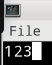
\includegraphics{figures/fig28.png}
					\end{figure}
				
					\item 在input目录下创建b.txt文件,添加如下内容:\\
					456
					
					\begin{figure}[H]
						\centering
						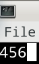
\includegraphics{figures/fig29.png}
					\end{figure}
					
					\item 在input目录下创建c.txt文件,添加如下内容:\\
					789
					
					\begin{figure}[H]
						\centering
						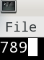
\includegraphics{figures/fig30.png}
					\end{figure}
				\end{enumerate}
			
				代码逻辑:
				\begin{enumerate}
					\item 获取HDFS文件系统对象FileSystem。
					\item 在HDFS根目录创建merge.txt文件。
					\item 获取本地文件系统。
					\item 获取本地文件系统文件列表集合。
					\item 迭代遍历文件列表获取数据并进行数据拷贝。
					\item 关闭资源。
					\begin{figure}[H]
						\centering
						
\includegraphics[width=4.5in]{figures/fig31.png}
					\end{figure}
				\end{enumerate}
			
				查看结果:通过命令查看HDFS根目录下的merge.txt文件。
				\begin{figure}[H]
					\centering
					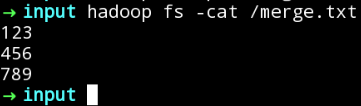
\includegraphics{figures/fig32.png}
				\end{figure}
	
	\section{结果分析}
		HDFS的Java API操作主要通过调用现成的包内函数方法来实现。
					
	\section{困难解决}
		本次实验较为简单,没有遇到困难。
	
	\section{心得体会}
		做完本次实验,除了掌握了实验目的部分中所有内容的收获之外,我还有以下几点心得体会:
		\begin{itemize}
			\item 实践并掌握了HDFS中用Java API进行创建目录和上传、遍历、下载合并文件等操作;
			\item 对比分析了HDFS中用Java API和Shell命令对文件进行上传查看、修改删除等操作的异同点。
		\end{itemize}
	
%\end{sloppypar}
\end{document}
\endinput